%==============================================================

\section{Big Data}\label{bdf}

After evaluating different data sources presenting various methods to extract and process different audio features, the following section describes the data analysis with big data processing frameworks like Apache Spark \cite{spark} and Hadoop \cite{hadoop}. Most of the basic information on Hadoop and Spark in the next few sections are taken from the book "Data Analytics with Spark using Python" by Jeffrey Aven, which gives a very comprehensible and practical introduction to the field of big data processing with PySpark \cite{sparkbook1}. Later, Section \ref{bds1} deals with the implementation of the various similarity measurements with Spark, the handling of larger amounts of data, runtime analysis and the combination of multiple similarity measurements, while Chapter \ref{bds2} gives a short overview over the achieved results using the big data framework to compare audio features. 

\subsection{Hadoop}

With the ever-growing availability of huge amounts of high-dimensional data, the need for toolkits and efficient algorithms to handle these grew as well over the past years. One key to handle big data problems is the use of parallelism.\\
Search engine providers like Google and Yahoo firstly ran into the problem of using "internet-scale" data in the early 2000s when being faced with the problem of storing and processing the ever-growing amount of indexes from documents on the internet. In 2003, Google presented their white paper called "The Google File System" \cite{gfs}. MapReduce is a programming paradigm introduced by Google as an answer to the problem of internet-scale data and dates back to 2004 when the paper "MapReduce: Simplified Data Processing on Large Clusters" was published \cite{mapreduce1}.\\ 
Doug Cutting and Mike Cafarella worked on a web crawler project called "Nutch" during that time. Inspired by the two papers Cutting incorporated the storage and processing principles from Google, leading to what we know as Hadoop today. Hadoop joined the Apache Software Foundation in 2006. \cite[p. 6]{sparkbook1}\\ 
Hadoop is a scalable solution able to run on large computer clusters. It does not necessarily require a supercomputing environment and is able to run on clusters of lower-cost commodity hardware. The data is stored redundantly on multiple nodes with a configurable replication factor defining how many copies of each data chunk are stored redundantly on other nodes. This enables an error management where faulty operations can simply be restarted.\\
Hadoop is based on the idea of data locality. In contrast to the usual approach, where the data is requested from its location and transferred to a remote processing system or host, Hadoop brings the computation to the data instead. This minimizes the problem of data transfer times over the network at compute time when working with very large-scale data/ big data. One prerequisite is that the operations on the data are independent of each other. Hadoop follows this approach called "shared nothing", where data is processed locally on many nodes at the same time in parallel by splitting the data into independent, small subsets without the need for communication with other nodes. Additionally, Hadoop is a schemaless (schema-on-read) system which means that it is able to store and process unstructured, semi-structured (JSON, XML), or well structured data (relational database). \cite[p. 7]{sparkbook1}\\
To make all this possible, Hadoop relies on its core components YARN (Yet Another Resource Negotiator) as the processing and resource scheduling subsystem and the Hadoop Distributed File System (HDFS) as Hadoop's data storage subsystem\\

\subsubsection{MapReduce}

Figure \ref{mapred} shows the basic scheme of a MapReduce program. 

\FloatBarrier
\begin{figure}[htbp]
	\centering
	\framebox{\parbox{1\textwidth}{ 
	%Image based on: https://commons.wikimedia.org/wiki/File:Mapreduce.png
	\begin{tikzpicture}[node distance = 4cm][every node/.style={thick}]
	  \colorlet{coul0}{orange!20} \colorlet{coul1}{blue!20} \colorlet{coul2}{red!20} \colorlet{coul3}{green!20}
	  \tikzstyle{edge}=[->, very thick]
	  \draw[thick, fill=violet!30] (-1, -2) rectangle node[rotate=90] {\textbf{Input data}} (0,2);
	  \foreach \i in {0,1,2,3} {
	    \node[draw, fill=coul\i, xshift=2em] (data\i) at (1.5, 1.5 - \i) {Input};
	    \node[ellipse, draw, fill=cyan!20, xshift=2em] (map\i) at (3.5, 1.5 - \i) {\textsf{Map}};
	    \draw[edge] (0,0) -- (data\i.west);
	    \draw[edge] (data\i) -- (map\i);
	  }
	  \node[draw, minimum height=2cm, fill=purple!30, xshift=7em] (resultat) at (10, 0) {\textbf{Results}};
	  \foreach \i in {0,1,2} {
	    \node[draw, fill=yellow!20, minimum width=2cm, xshift=4em] (paire\i) at (5.5, 1.5 - \i*1.5) {\begin{minipage}{1cm}Tuples \centering $\langle k,v \rangle$\end{minipage}};
	    \node[ellipse, draw, fill=cyan!20, xshift=6em] (reduce\i) at (7.5, 1.5 - \i*1.5) {\textsf{Reduce}};
	    \draw[edge] (paire\i) -- (reduce\i);
	    \draw[edge] (reduce\i.east) -- (resultat);
	  }
	  %paire
	  \draw[edge] (map0.east) -- (paire0.west); \draw[edge] (map0.east) -- (paire1.west);
	  \draw[edge] (map1.east) -- (paire0.west); \draw[edge] (map1.east) -- (paire2.west);
	  \draw[edge] (map2.east) -- (paire1.west); \draw[edge] (map2.east) -- (paire0.west);
	  \draw[edge] (map3.east) -- (paire1.west); \draw[edge] (map3.east) -- (paire2.west);
	\end{tikzpicture}
	}}
	\caption{MapReduce \cite{mapred1im}}
	\label{mapred}
\end{figure}
\FloatBarrier

\noindent In the first stage, the input data is split into chunks and distributed over the nodes of a cluster. This is usually managed by a distributed file system like the HDFS. One master node stores the addresses of all data chunks.\\
The data is then fed into the mappers which operate on the input data and finally transforms the input into key-value tuples.\\
In an intermediate step the key-value pairs are usually grouped by their keys before being fed into the reducers. The reducers apply another method to all tuples with the same key.\\
The amount of key-value pairs at the output from all mappers divided by the number of input files is called "replication rate" ($r$). The highest count of values for one key being fed into a reducer can be denoted as $q$ (reducer size). Usually, there is a trade-off between a high replication rate $r$ and small reducer size $q$ (highly parallel with more network traffic) or small $r$ and larger $q$ (less network traffic but worse parallelism due to an overall smaller reducer count).

\subsection{Spark}\label{sparksec}

Hadoop as a big data processing framework has a few downsides compared to other, newer options like Spark. The Spark project was started in 2009 and was created as a part of the Mesos research project. It was developed as an alternative to the implementation of MapReduce in Hadoop. Spark is written in the programming language Scala and runs in Java Virtual Machines (JVM) but also provides native support for programming interfaces in Python, Java and R. One major advantage compared to Hadoop is the efficient way of caching intermediate data to the main memory instead of writing it the hard drive. While Hadoop has to read all data from the disk and writes all results back to the disk, Spark can efficiently take advantage of the RAM from the different nodes, making it suitable for interactive queries and iterative machine learning operations. To be able to offer these kinds of in-memory operations Spark uses a structure called "Resilient Distributed Dataset" (RDD). \cite[p. 13]{sparkbook1}\\ 
Figure \ref{dataloc} shows the simplified architecture of a compute cluster running Spark. 

\begin{figure}[htbp]
	\centering
	\framebox{\parbox{1\textwidth}{ 
	\begin{tikzpicture}
	\tikzstyle{bigbox} = [draw=blue!60, blur shadow={shadow blur steps=5}, minimum size=2cm, thick, fill=blue!10, rounded corners, rectangle]
	\tikzstyle{box} = [draw=black!40!blue, minimum size=0.6cm, rounded corners,rectangle, fill=blue!50]
	\tikzstyle{box2} = [draw=black!60!blue, minimum size=0.6cm, rounded corners,rectangle, fill=blue!10]
	\tikzstyle{box3} = [draw=blue!80, minimum size=0.6cm, rounded corners,rectangle, fill=blue!10]
	\node[server](server 1){};
	\node[server, right of= server 1, xshift=3cm](server 2){};
	\node[server, right of= server 2, xshift=3cm](server 3){};
	\node[rack switch, above of=server 2,xshift=0.1cm,yshift=0.25cm]
	  (rack switch 1){};
   	\node[box, above of=rack switch 1, xshift=0cm, yshift=0.95cm](cm){Cluster Manager}; 
	\begin{pgfonlayer}{background}
		\node[bigbox, yshift=-0.25cm, xshift=-0.01cm] [fit = (cm)](ma){\\ \ \\Master};
	\end{pgfonlayer}
   	\node[server, above of=ma, yshift=0.75cm](servermaster){};
 	\node[box, above of=servermaster, xshift=0cm, yshift=1.25cm](sc){SparkSession}; 
  	\begin{pgfonlayer}{background}
  		\node[bigbox, yshift=-0.25cm, xshift=-0.01cm] [fit = (sc)](dr){\\ \ \\Driver};
  	\end{pgfonlayer}
	\node[box, below of=server 3, xshift=-3.25em, yshift=-0.25cm](e1){Executor 1};
	\node[box, below of=server 3, xshift=3.25em, yshift=-0.25cm](e2){Executor 2};
	\node[box, below of=server 2, xshift=0em, yshift=-0.25cm](e3){Executor 3};
	\node[box, below of=server 1, xshift=-3.25em, yshift=-0.25cm](e4){Executor 4};
	\node[box, below of=server 1, xshift=3.25em, yshift=-0.25cm](e5){Executor 5};
	\begin{pgfonlayer}{background}
		\node[bigbox, yshift=-0.35cm, xshift=-0.01cm] [fit = (e1)](mem1){\\ \ \\Memory};
	\end{pgfonlayer}
	\begin{pgfonlayer}{background}
		\node[bigbox, yshift=-0.35cm, xshift=0.01cm] [fit = (e2)](mem2){\\ \ \\Memory};
	\end{pgfonlayer}
	\begin{pgfonlayer}{background}
		\node[bigbox, yshift=-0.35cm] [fit = (e3)](mem3){\\ \ \\Memory};
	\end{pgfonlayer}
	\begin{pgfonlayer}{background}
		\node[bigbox, yshift=-0.35cm, xshift=-0.01cm] [fit = (e4)](mem4){\\ \ \\Memory};
	\end{pgfonlayer}
	\begin{pgfonlayer}{background}
		\node[bigbox, yshift=-0.35cm, xshift=0.01cm] [fit = (e5)](mem5){\\ \ \\Memory};
	\end{pgfonlayer}
	\node[box2, below of=mem1, yshift=-0.01cm](t1){Task 1};
	\node[box2, below of=mem2, yshift=-0.01cm](t2){Task 2};
	\node[box2, below of=mem3, yshift=-0.01cm](t3){Task 3};
	\node[box2, below of=mem4, yshift=-0.01cm](t4){Task 4};
	\node[box2, below of=mem5, yshift=-0.01cm](t5){Task 5};
	\node[box2, below of=t2, yshift=0.3cm](t6){Task 6};
	\node[box2, below of=t4, yshift=0.3cm](t7){Task 7};
	\node[box2, below of=t5, yshift=0.3cm](t8){Task 8};
	\draw[thick,black!60!green] (t2.south)--(t6);	
	\draw[thick,black!60!green] (t4.south)--(t7);	
	\draw[thick,black!60!green] (t5.south)--(t8);	
	\draw[thick,darkgray!10!gray] (servermaster.north)--(dr.south);
	\draw[thick,darkgray!10!gray] (servermaster.south)--(ma.north);
	\draw[thick,darkgray!10!gray] (ma.south)--(rack switch 1.north);
	\draw[thick,darkgray!10!gray] (server 1.north)--(rack switch 1);
	\draw[thick,darkgray!10!gray] (server 2.north)--(rack switch 1);
	\draw[thick,darkgray!10!gray] (server 3.north)--(rack switch 1);
	\draw[thick,darkgray!10!gray] (server 3.south)--(e1);	
	\draw[thick,darkgray!10!gray] (server 3.south)--(e2);	
	\draw[thick,darkgray!10!gray] (server 2.south)--(e3);	
	\draw[thick,darkgray!10!gray] (server 1.south)--(e4);	
	\draw[thick,darkgray!10!gray] (server 1.south)--(e5);	
	% = = = = = = = = = = = = = = = =
	% Labels
	% = = = = = = = = = = = = = = = =
	\node[box3, xshift=-6.1cm,yshift=0.3cm,left of = sc,align=left](lev1){\textbf{Main Program}};
	\node[box3, xshift=-6.25cm,yshift=0.3cm,left of = servermaster,align=left](lev2){\textbf{Master Node}};
	\node[box3, xshift=-5.85cm,yshift=0.3cm,left of = cm,align=left](lev3){\textbf{Cluster Manager}};	
	\node[box3, xshift=-6.9cm,yshift=0.3cm,left of = rack switch 1,align=left](lev4){\textbf{Switch}};
	\node[box3, xshift=-2.185cm,yshift=0.3cm,left of = server 3,align=left](lev5){\textbf{Worker Nodes}};
	\node[box3, xshift=-1.325cm,yshift=0.3cm,left of = e1,align=left](lev6){\textbf{Executors}};
	\end{tikzpicture}
	}}
	\caption{Spark Cluster}
	\label{dataloc}
\end{figure}

\noindent The core components of a Spark application are the Driver, the Master, the Cluster Manager, and the Executors. The Driver is the process where clients submit their applications to. It is responsible for the planning and execution of a Spark program and returns status logs and results to the clients. It can be located on a remote client or on a node in the cluster. The SparkSession is created by the Driver and represents a connection to a Spark cluster. The SparkContext and SparkConf as child objects of the SparkSession contain the necessary information to configure the cluster parameters, e.g., the number of CPU cores and memory assigned to the executors and the number of executors that get spawned overall on the cluster. Up until version 2.0 entry points for Spark applications included the SparkContext, SQLContext, HiveContext, and StreamingContext. In more recent versions these were combined into one SparkSession object providing a single entry point.
The execution of the Spark application is planned and directed acyclic graphs (DAG) are created by the Spark Driver. The nodes of these DAGs represent transformational or computational steps on the data. These DAGs can be visualized using the Spark application UI typically running on port 4040 of the Driver node. The Spark application UI is a useful tool to improve the performance of Spark applications and for debugging, as it also gives information about the computation time of the distinct tasks within a Spark program. \cite[pp. 45 ff]{sparkbook1}\\
Two examples of information provided by the Spark application UI are shown in Figure \ref{appui}.\\

\begin{figure}[htbp]
	\captionsetup[subfigure]{justification=centering}
	\centering
	\framebox{\parbox{1\textwidth}{
	\begin{subfigure}{.5\textwidth}
		\captionsetup{justification=centering}
		\captionsetup[subfigure]{justification=centering}
		\centering
		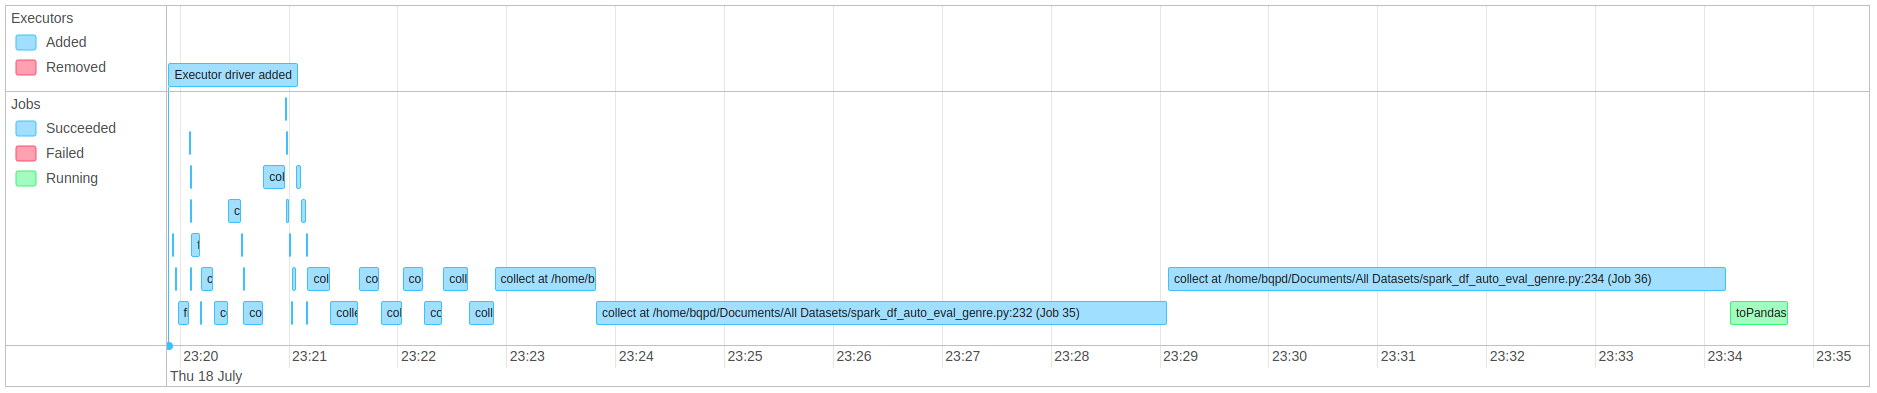
\includegraphics[scale=0.23]{Images/Spark/df_slow_chroma.png}
		\caption{\noindent Event Timeline}
		\label{sui2}
	\end{subfigure}%
	
	\begin{subfigure}{.5\textwidth}
	\captionsetup{justification=centering}
	\captionsetup[subfigure]{justification=centering}
	\centering
	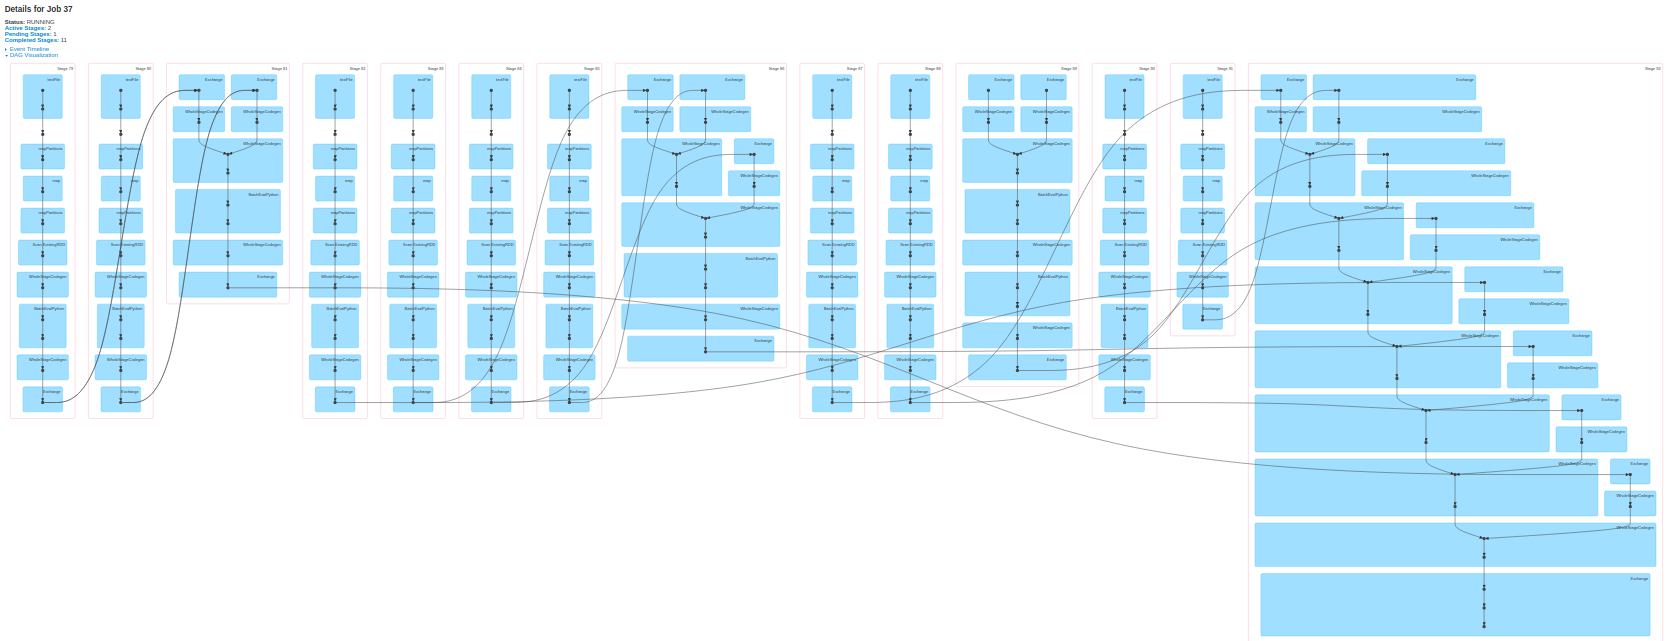
\includegraphics[scale=0.26]{Images/Spark/toPandasDag.png}
	\caption{\noindent DAG}
	\label{sui3}
	\end{subfigure}% 		
	}}
	\caption{Spark Application UI}
	\label{appui}
\end{figure}
\FloatBarrier

\noindent The Workers are the nodes in the cluster where the actual computation of the Spark DAG tasks take place. As defined within the SparkConf, the Worker nodes spawn a finite or fixed number of Executors that reserve CPU and memory resources and run in parallel. The Executors are hosted in JVMs on the Workers. Finally, the Spark Master and the Cluster Manager are the processes that monitor, reserve and allocate the resources for the executors. Spark can work on top of various Cluster Managers like Apache Mesos, Hadoop, YARN, and Kubernetes. Spark can also work in standalone mode, where the Spark Master also takes control of the Cluster Managers' tasks. If Spark is running on top of a Hadoop cluster, it uses the YARN ResourceManager as the Cluster Manager and the ApplicationMaster as the Spark Master. The ApplicationMaster is the first task allocated by the ResourceManager and negotiates the resources (containers) for the Executors and makes them available to the Driver. \cite[pp. 49 ff]{sparkbook1}\\
When running on top of a Hadoop installation, Spark can additionally take advantage of the HDFS by reading data directly out of it.\\

\subsubsection{Cluster Configuration and Execution}\label{cconfexp}


There are multiple options of passing a Spark programm to the cluster. The first one is to use a spark shell e.g. by calling \lstinline{pyspark} when working with the Spark Python API or \lstinline{spark-shell} (Scala). If the interactive option of using a spark shell is chosen, a SparkSession is automatically created and exited once the spark shell gets closed. 
Alternatively the Spark application can be passed to the cluster directly using \lstinline{spark-submit application.py -options} (Python).
As mentioned previously the configuration of the Spark cluster can be changed. This can either be done by using a cluster configuration file (e.g. spark-defaults.conf), by submitting the parameters as arguments passed to pyspark, spark-console or spark-submit or by directly setting the configuration properties inside the Spark application code (see Code Snippet \ref{lst:cconf})\\


\begin{pythonCode}[frame=single,label={lst:cconf},caption={Example cluster configuration Python},captionpos=b]
confCluster = SparkConf().setAppName("MusicSimilarity Cluster")
confCluster.set("spark.driver.memory", "1g")
confCluster.set("spark.executor.memory", "1g")
confCluster.set("spark.executor.memoryOverhead", "500m")
#Sum of the driver or executor memory plus the driver or executor memory overhead is always less than the value of yarn.nodemanager.resource.memory-mb
#confCluster.set("yarn.nodemanager.resource.memory-mb", "8192")
confCluster.set("spark.yarn.executor.memoryOverhead", "512")
#set cores of each executor and the driver -> less than avail -> more executors spawn
confCluster.set("spark.executor.cores", "1")
confCluster.set("spark.shuffle.service.enabled", "True")
confCluster.set("spark.dynamicAllocation.enabled", "True")
confCluster.set("spark.dynamicAllocation.minExecutors", "4")
confCluster.set("spark.dynamicAllocation.maxExecutors", "8")
confCluster.set("yarn.nodemanager.vmem-check-enabled", "false")
sc = SparkContext(conf=confCluster)
sqlContext = SQLContext(sc)
spark = SparkSession.builder.master("cluster").appName("MusicSimilarity").
	getOrCreate()
\end{pythonCode}

\subsubsection{Spark Advantages}

For this thesis, the programming language of choice is Python. With its high-level Python API, Spark applications can take advantage of commonly known and widely used Python libraries such as Numpy or Scipy. It also contains its own powerful libraries like the Spark ML library for machine learning applications or GraphX for the work with large graphs.\\ 
Spark can be used in combination with SQL (e.g., the Hive project) and NoSQL Systems like Cassandra and HBase. Spark SQL enables the transformation of RDDs to well structured DataFrames. The DataFrame concept is later used in Section \ref{bds1}.\\
One other important concept Spark uses is its lazy evaluation or lazy execution. Spark differentiates between data transformations (e.g. \lstinline{filter()}, \lstinline{join()}, and \lstinline{map()}) and actions (e.g. \lstinline{take} or \lstinline{count}). The actual processing and transformation of data is deferred until an action is called. In the example Code Snippet \ref{lst:lev} the \lstinline{map()} and \lstinline{filter()} transformations are only executed once the \lstinline{count()} action is called. Only then a DAG is created together with logical and physical execution plans and the tasks are distributed across the Executors. The lazy evaluation allows Spark to combine as many operations as possible which may lead to a drastic reduction of processing stages and data shuffling (data transferred between executors) and thus reducing unnecessary overhead and data/ network traffic. But the lazy execution has to be kept in mind during debugging and performance testing. \cite[p.73]{sparkbook1}

\begin{pythonCode}[frame=single,label={lst:lev},caption={Lazy evaluation},captionpos=b]
chroma = sc.textFile("features.txt").repartition(repartition_count)
chroma = chroma.map(lambda x: x.split(';'))
chroma = chroma.filter(lambda x: x[0] == "OrbitCulture_SunOfAll.mp3")
chroma = chroma.count()
\end{pythonCode}

\noindent Another important part of Spark is its ability to process streaming data. While Hadoop is good at batch processing very large datasets but rather slow when it comes to iterative tasks on the same data due to its persistent write operations to the hard drive, Spark outperforms Hadoop with its ability to use RDDs and the main memory during iterative tasks. 
With Spark streaming the possibility to process data streams, e.g., from social networks, in real-time is given.\\
The combination of batch- and stream-processing methods is called "Lambda architecture" in data science literatur. It describes a data-processing architecture consisting of a Batch-Layer, a Speed-Layer for real-time processing and a Serving-Layer managing the data \cite[pp. 8 f]{nextgenbig}. Spark offers the possibility to take care of both, batch- and stream-processing jobs. Combined with other frameworks like the Apache SMACK stack (Spark, Mesos, Akka, Cassandra, and Kafka), Spark offers manyfold possibilities for high-throughput big data processing \cite[p. 5]{smack}.\\
This thesis preliminary only focuses on batch processing and finding similar items. But the possibility to pass song titles in real-time to Spark and getting recommendation lists of similar songs in a few seconds in return could be a long-term goal of future work.\\

\subsection{Music Similarity with Big Data Frameworks}

Given the short introduction to big data frameworks, the decision to use Spark for the computation of the similarities between audio features can be justified as follows.\\
The computation of the "one-to-many-item" similarity follows the shared nothing approach of Spark. All of the features from different songs are independent of each other, and the distances can be computed in parallel. Only the scaling of the result requires an aggregation of maximum and minimum values. And to return the top results, some kind of sorting has to be performed. But apart from these operations that require data shuffling, all the features can be distributed on a cluster and the similarity to one broadcasted song can be calculated independently, following the data locality principle. This offers a fully scalable solution for very large datasets. Additionally, Spark enables efficient ways to cache the audio feature data into the main memory. Under the prerequisite that the sum of all features from all songs fit into the main memory of the cluster, interactive consecutive song requests could be answered without the need of reading the features from the hard drive every time.
One limitation is, that Spark itself is unable to read and handle audio files. So the feature extraction itself has to be performed separately, and only the extracted features are loaded into the cluster and processed with Spark. The feature extraction process is later described in Section \ref{simmet}.\\
The similarities can be calculated as "one-to-many-items" similarities. That means that for only one song at a time the similarities to all other songs have to be calculated. This is the approach investigated in this thesis. The other option would be to pre-calculate a full similarity matrix (All-pairs similarity). But looking at large-scale datasets with millions of songs this would take a considerable amount of time. A combination of both approaches would be to calculate the similarities for one song request at a time but store these similarities int a sparse similarity matrix once they got computed, to speed up subsequent requests of the same songs. But this won't be the topic of this thesis.\\ 
To clarify the usage of a few terms further throughout this thesis (especially later in Section \ref{bds1}), the term "song request" describes the song title passed to the recommendation engine to estimate the similarities. The terms similarities and distances are used synonymously in this thesis because all the similarity estimations are based on distances between feature vectors of different feature types (see equation \eqref{eq:distsim}). The smaller the distance $d(x, y)$ between the audio features of two songs $x$ and $y$ is, the greater gets the similarity $sim(x, y)$ between these songs.\\
\begin{equation} \label{eq:distsim}
%p (v \vert \lambda)=\sum_{i=1}^{M}w_iN(v \vert \mu_i,\sum_i) \label{prob}
sim(x, y) = \frac{1}{d(x, y)}
\end{equation}

